%%
%% This is file `sample-acmsmall.tex',
%% generated with the docstrip utility.
%%
%% The original source files were:
%%
%% samples.dtx  (with options: `all,journal,bibtex,acmsmall')
%% 
%% IMPORTANT NOTICE:
%% 
%% For the copyright see the source file.
%% 
%% Any modified versions of this file must be renamed
%% with new filenames distinct from sample-acmsmall.tex.
%% 
%% For distribution of the original source see the terms
%% for copying and modification in the file samples.dtx.
%% 
%% This generated file may be distributed as long as the
%% original source files, as listed above, are part of the
%% same distribution. (The sources need not necessarily be
%% in the same archive or directory.)
%%
%%
%% Commands for TeXCount
%TC:macro \cite [option:text,text]
%TC:macro \citep [option:text,text]
%TC:macro \citet [option:text,text]
%TC:envir table 0 1
%TC:envir table* 0 1
%TC:envir tabular [ignore] word
%TC:envir displaymath 0 word
%TC:envir math 0 word
%TC:envir comment 0 0
%%
%%
%% The first command in your LaTeX source must be the \documentclass
%% command.
%%
%% For submission and review of your manuscript please change the
%% command to \documentclass[manuscript, screen, review]{acmart}.
%%
%% When submitting camera ready or to TAPS, please change the command
%% to \documentclass[sigconf]{acmart} or whichever template is required
%% for your publication.
%%
%%
\documentclass[acmsmall]{acmart}

%%
%% \BibTeX command to typeset BibTeX logo in the docs
\AtBeginDocument{%
  \providecommand\BibTeX{{%
    Bib\TeX}}}

%% Rights management information.  This information is sent to you
%% when you complete the rights form.  These commands have SAMPLE
%% values in them; it is your responsibility as an author to replace
%% the commands and values with those provided to you when you
%% complete the rights form.
\setcopyright{acmlicensed}
\copyrightyear{2024}
\acmYear{2024}
\acmDOI{XXXXXXX.XXXXXXX}


%%
%% These commands are for a JOURNAL article.
\acmJournal{JACM}
\acmVolume{37}
\acmNumber{4}
\acmArticle{111}
\acmMonth{8}

%%
%% Submission ID.
%% Use this when submitting an article to a sponsored event. You'll
%% receive a unique submission ID from the organizers
%% of the event, and this ID should be used as the parameter to this command.
%%\acmSubmissionID{123-A56-BU3}

%%
%% For managing citations, it is recommended to use bibliography
%% files in BibTeX format.
%%
%% You can then either use BibTeX with the ACM-Reference-Format style,
%% or BibLaTeX with the acmnumeric or acmauthoryear sytles, that include
%% support for advanced citation of software artefact from the
%% biblatex-software package, also separately available on CTAN.
%%
%% Look at the sample-*-biblatex.tex files for templates showcasing
%% the biblatex styles.
%%

%%
%% The majority of ACM publications use numbered citations and
%% references.  The command \citestyle{authoryear} switches to the
%% "author year" style.
%%
%% If you are preparing content for an event
%% sponsored by ACM SIGGRAPH, you must use the "author year" style of
%% citations and references.
%% Uncommenting
%% the next command will enable that style.
%%\citestyle{acmauthoryear}

% Language setting
% Replace `english' with e.g. `spanish' to change the document language
\usepackage[english]{babel}

% Useful packages
\usepackage{amsmath}
\usepackage{graphicx}
%\usepackage{amssymb}
\usepackage{array}
%\usepackage[colorlinks=true, allcolors=blue]{hyperref}

%%
%% end of the preamble, start of the body of the document source.
\begin{document}

%%
%% The "title" command has an optional parameter,
%% allowing the author to define a "short title" to be used in page headers.
\title{Finch: A Datastructure-Driven Array Programming Language}

%%
%% The "author" command and its associated commands are used to define
%% the authors and their affiliations.
%% Of note is the shared affiliation of the first two authors, and the
%% "authornote" and "authornotemark" commands
%% used to denote shared contribution to the research.
\author{Willow Ahrens}
\affiliation{%
  \institution{MIT CSAIL}
  \city{Cambridge}
  \state{Massachusetts}
  \country{USA}}
\email{willow@csail.mit.edu}

\author{Teo Collins}
\affiliation{%
  \institution{MIT CSAIL}
  \city{Cambridge}
  \state{Massachusetts}
  \country{USA}}
\email{teoc@mit.edu}

\author{Radha Patel}
\affiliation{%
  \institution{MIT CSAIL}
  \city{Cambridge}
  \state{Massachusetts}
  \country{USA}}
\email{rrpatel@mit.edu}

\author{Kyle Deeds}
\affiliation{%
  \institution{University of Washington}
  \city{Seattle}
  \state{Washington}
  \country{USA}}
\email{kdeeds@cs.washington.edu}

\author{Changwan Hong}
\affiliation{%
  \institution{MIT CSAIL}
  \city{Cambridge}
  \state{Massachusetts}
  \country{USA}}
\email{changwan@mit.edu}

\author{Saman Amarasinghe}
\affiliation{%
  \institution{MIT CSAIL}
  \city{Cambridge}
  \state{Massachusetts}
  \country{USA}}
\email{saman@csail.mit.edu}

%%
%% By default, the full list of authors will be used in the page
%% headers. Often, this list is too long, and will overlap
%% other information printed in the page headers. This command allows
%% the author to define a more concise list
%% of authors' names for this purpose.
\renewcommand{\shortauthors}{Ahrens et al.}

%%
%% The abstract is a short summary of the work to be presented in the
%% article.
\begin{abstract}
From FORTRAN to Numpy, arrays have revolutionized how we express computation.  Arrays are the highest-performing datastructure with a long history of investment and innovation, from hardware support to compiler technology.  However, arrays can only handle dense rectilinear integer grids. Real world arrays often contain underlying structure, such as sparsity, runs of repeated values, or symmetry. We describe a compiler, Finch, which adapts existing programs and interfaces to the structure and sparsity of the inputs. Finch enables programmers to capture complex, real-world data scenarios with the same productivity they expect from dense arrays. Our approach enables new loop optimizations across multiple domains, unifying techniques such as sparse tensors, databases, and lossless compression. 
\end{abstract}

%%
%% The code below is generated by the tool at http://dl.acm.org/ccs.cfm.
%% Please copy and paste the code instead of the example below.
%%
\begin{CCSXML}
<ccs2012>
 <concept>
  <concept_id>00000000.0000000.0000000</concept_id>
  <concept_desc>Do Not Use This Code, Generate the Correct Terms for Your Paper</concept_desc>
  <concept_significance>500</concept_significance>
 </concept>
 <concept>
  <concept_id>00000000.00000000.00000000</concept_id>
  <concept_desc>Do Not Use This Code, Generate the Correct Terms for Your Paper</concept_desc>
  <concept_significance>300</concept_significance>
 </concept>
 <concept>
  <concept_id>00000000.00000000.00000000</concept_id>
  <concept_desc>Do Not Use This Code, Generate the Correct Terms for Your Paper</concept_desc>
  <concept_significance>100</concept_significance>
 </concept>
 <concept>
  <concept_id>00000000.00000000.00000000</concept_id>
  <concept_desc>Do Not Use This Code, Generate the Correct Terms for Your Paper</concept_desc>
  <concept_significance>100</concept_significance>
 </concept>
</ccs2012>
\end{CCSXML}

\ccsdesc[500]{Do Not Use This Code~Generate the Correct Terms for Your Paper}
\ccsdesc[300]{Do Not Use This Code~Generate the Correct Terms for Your Paper}
\ccsdesc{Do Not Use This Code~Generate the Correct Terms for Your Paper}
\ccsdesc[100]{Do Not Use This Code~Generate the Correct Terms for Your Paper}

%%
%% Keywords. The author(s) should pick words that accurately describe
%% the work being presented. Separate the keywords with commas.
\keywords{Do, Not, Us, This, Code, Put, the, Correct, Terms, for,
  Your, Paper}

\received{20 February 2007}
\received[revised]{12 March 2009}
\received[accepted]{5 June 2009}

%%
%% This command processes the author and affiliation and title
%% information and builds the first part of the formatted document.
\maketitle

\section{Introduction}

%- Fortran supported lots of control structures, no data structures, just dense arrays.
%
%- We tried to emulate complex data using only dense arrays but with complicated control structures.
%
%- Recently, people tried to build frameworks to support structured data, but gave up a lot of program side
%
%- We’re bringing these together, both need to work together.
\subsection{Contributions}

\begin{enumerate}
\item A rich structured array programming language with for-loops
and complex control flow constructs at the same level of productivity
of dense arrays. To our knowledge, the Finch programming language is the first
to support if-conditions, early breaks, and multiple left hand sides over
structured data, as well as complex accesses such as affine indexing or scatter/gather.
\item More complex array structures than ever before. A complete level-by-level
structure-description language for expressing the structure of data
hierarchically. The first such set of formats to efficiently capture banded,
triangular, run-length-encoded, or sparse datasets, and any combination thereof.
\item The Finch compiler specializes programs to data structures in a
predictable, deterministic approach, making it easier to search the complex
space of programs and datastructures to find an appropriate fit for a given
application. The tensor interface makes it easy to extend Finch to new level
formats. A unique tensor lifecycle model enables polymorphism by analyzing the
appropriate stages to insert simple, overloadable, interface functions such as
initialization or finalization. 
\item A high-level array programming language and fusion interface for
operations such as map, broadcast, or reduce that can be compiled to efficient
code using the previous loop-level abstractions.
\item We evaluate the productivity of our language in several case studies,
showing that Finch can be used to accelerate a wide range of applications, 
from classic operations such as spmv and spgemm, to more complex applications such as image processing and graph analytics.
We also demonstrate how Finch can fuse high-level operations to achieve a significant speedup over non-fused kernels.
%\item A complete set of level formats for expressing data patterns hierarchically in FiberTree-style decompositions. The first such set of formats to efficiently capture banded, triangular, run-length-encoded, or sparse-run-length-encoded datasets. The formats capture many use cases, from random updates to sequential construction.
%\item The Finch array language, mirroring simple for-loops with imperative code blocks and if-conditions. The first array programming language for the above data formats to support multiple outputs, affine indexing, and imperfectly-nested loops.
%\item Tensor lifecycles, a simple constraint on tensor reads and writes that elegantly restricts Finch programs to avoid complex data dependencies, and enables tensor polymorphism by providing implementers with well-defined functions to overload.
%\item Wrapper Tensors which modify existing datastructures and recombine them to support new patterns, such as affine indexing, padding, transposition, and slicing.
%\item Wrapper Levels which modify existing datastructures and enabling complex features such as atomic updates or contiguous versus separate allocation.
%\item We define the first mappings from the existing pydata/sparse array api high-level operations to low level finch notation
%\item <Performance Contributions>
\end{enumerate}

\begin{table}[h!]
\centering
\begin{tabular}{l|ccccc}
\textbf{Feature / Tool} & \textbf{Halide} & \textbf{Taco} & \textbf{Cora} & \textbf{Taichi} & \textbf{Finch} \\
\hline
Einsums and Contractions & \checkmark & \checkmark & \checkmark & \checkmark & \checkmark \\
Parallelism             & \checkmark & \checkmark & \checkmark & \checkmark & \checkmark \\
Multiple LHS            & \checkmark &            & \checkmark & \checkmark & \checkmark \\
Affine Indices          & \checkmark &            &            & \checkmark & \checkmark \\
Recurrence              & \checkmark &            &            &            &            \\
If-Conditions and Masks & \checkmark & \checkmark &            & \checkmark & \checkmark \\
Scatter Gather          & \checkmark &            &            & \checkmark & \checkmark \\
Early Break             &            & \checkmark &            &   \checkmark         & \checkmark \\
\end{tabular}
\caption{Feature support across various tools.}
\label{tab:features}
\end{table}

\begin{table}[h!]
\centering
\begin{tabular}{l|ccccc}
\textbf{Feature / Tool} & \textbf{Halide} & \textbf{Taco} & \textbf{Cora} & \textbf{Taichi} & \textbf{Finch} \\
\hline
Dense                    & \checkmark & \checkmark & \checkmark & \checkmark & \checkmark \\
Padded                   & \checkmark &            &            &            & \checkmark \\
One Sparse               &            & \checkmark &            & \checkmark & \checkmark \\
Sparse                   &            & \checkmark &            &            & \checkmark \\
Run-length               &            &            &            &            & \checkmark \\
Symmetric                &            &            &            &            & \checkmark \\
Regular Sparse Blocks    &            & \checkmark &            &            & \checkmark \\
Irregular Sparse Blocks  &            &            &            &            & \checkmark \\
Ragged                   &            &            & \checkmark &            & \checkmark \\
\end{tabular}
\caption{Support for various data structures across tools.}
\label{tab:data_structures}
\end{table}

\section{Background}
\subsection{Looplets}
\subsection{FiberTrees}

\subsection{Concordant Iteration}

\subsection{Protocols}

\section{The Finch Language}

\subsection{Syntax and Semantics}

\section{The Finch Compiler}

\subsection{Dimensionalization}

\subsection{Concordization}

\subsection{Bounds Analysis}

\subsection{Performance Warnings}

\subsection{Wrapperization}

\subsection{Simplification and Algebraic Transformations}

\section{The Tensor Interface}

\subsection{Tensor Lifecycle, Declare, Freeze, Thaw, Unfurl}

\subsection{Level Abstraction}
    
\begin{enumerate}
\item fibers
\item assembly
\item reassembly
\end{enumerate}

\subsection{Core Level Langage Primitives}
\begin{enumerate}
\item SparseList
\item SparseDict
\item ...
\end{enumerate}

\subsection{Wrapper Tensors}

\subsection{Scalars}

\subsubsection{Sparse Scalars}
\subsubsection{Early Break Scalars}

\section{The Finch High-Level API (Needs a Name)}

\subsection{Finch Logic}

\subsection{Finch Interpreter}

\subsection{Lowering}
\subsubsection{Heuristic Optimization}

\section{Evaluation}

\subsection{Data-Driven Performance Engineering}
\subsubsection{Sparse-Sparse Matrix Multiply}
Examples that demonstrate performance engineering in a datastructure-driven model

\subsubsection{SpMV}

%Here's a figure with spmv_performance_sorted_(faster_than_taco).png and spmv_performance_sorted_(slower_than_taco).png

\begin{figure}
    \begin{minipage}[t]{0.5\textwidth}
        \vspace{0pt} % Add this to ensure top alignment within minipage
        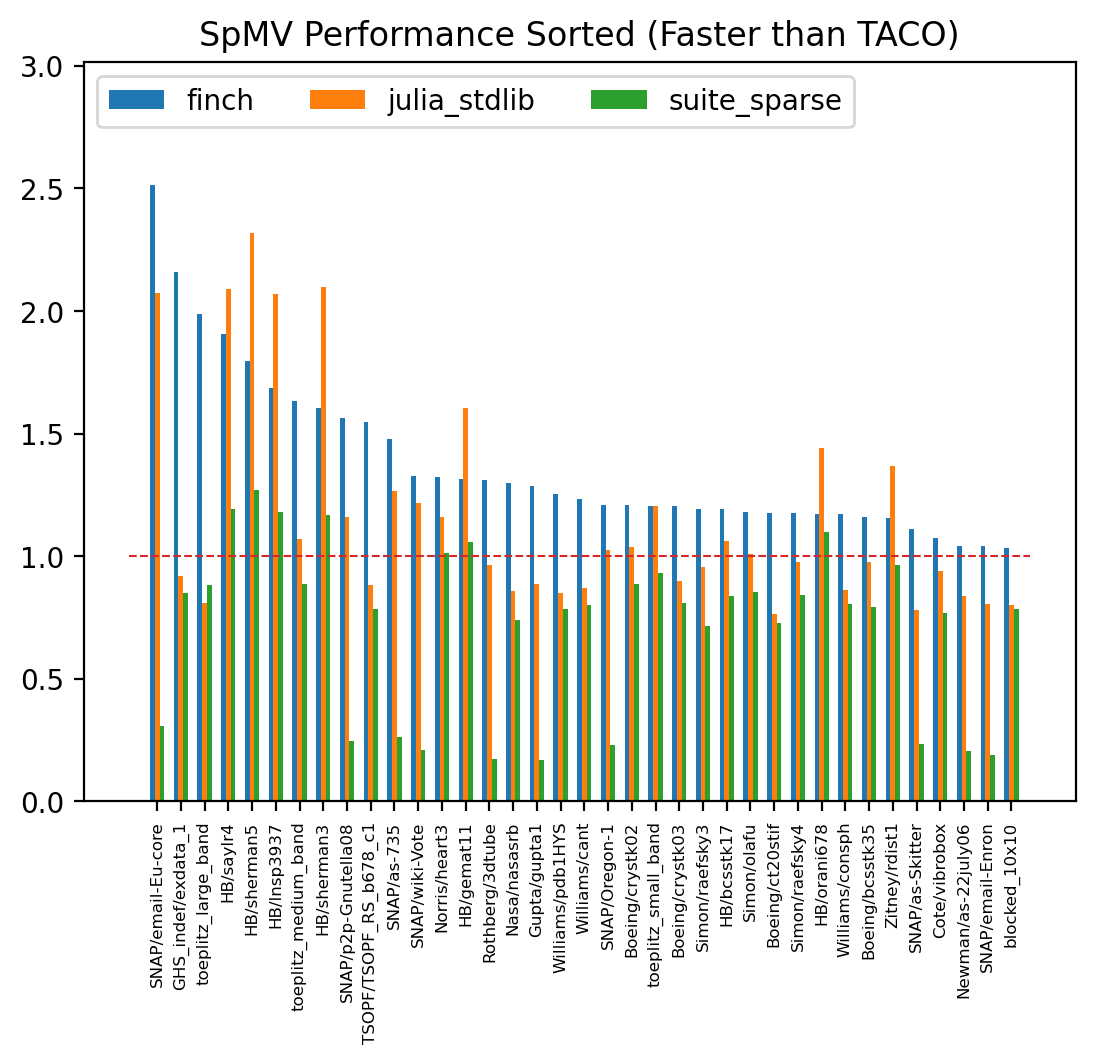
\includegraphics[width=\linewidth]{spmv_performance_sorted_(faster_than_taco).png}
    \end{minipage}%
    \begin{minipage}[t]{0.5\textwidth}
        \vspace{0pt} % Add this to ensure top alignment within minipage
        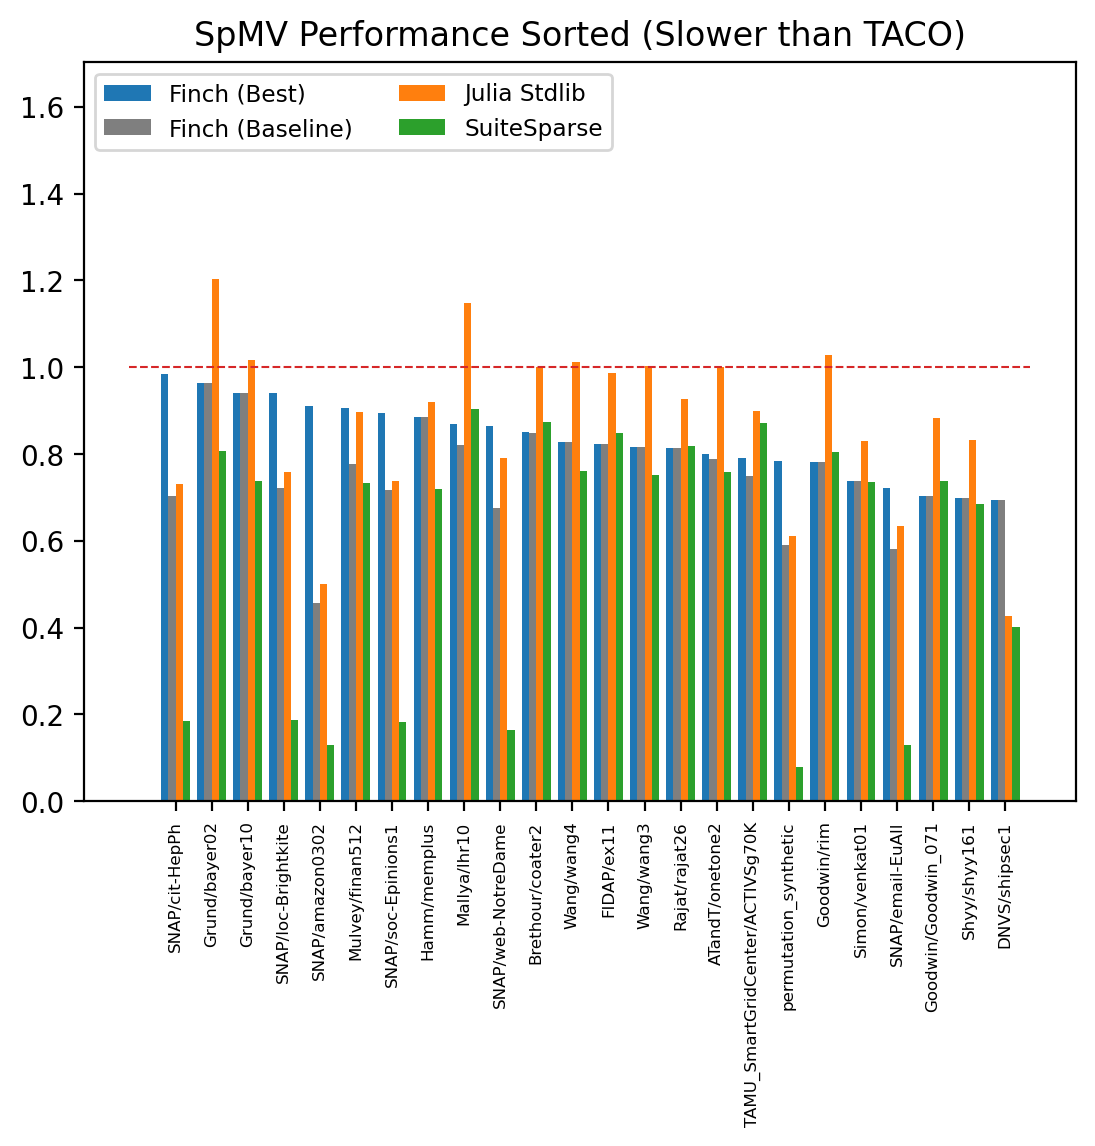
\includegraphics[width=\linewidth]{spmv_performance_sorted_(slower_than_taco).png}
    \end{minipage}
    \caption{Performance of SpMV across various tools.}
\end{figure}

\begin{figure}
    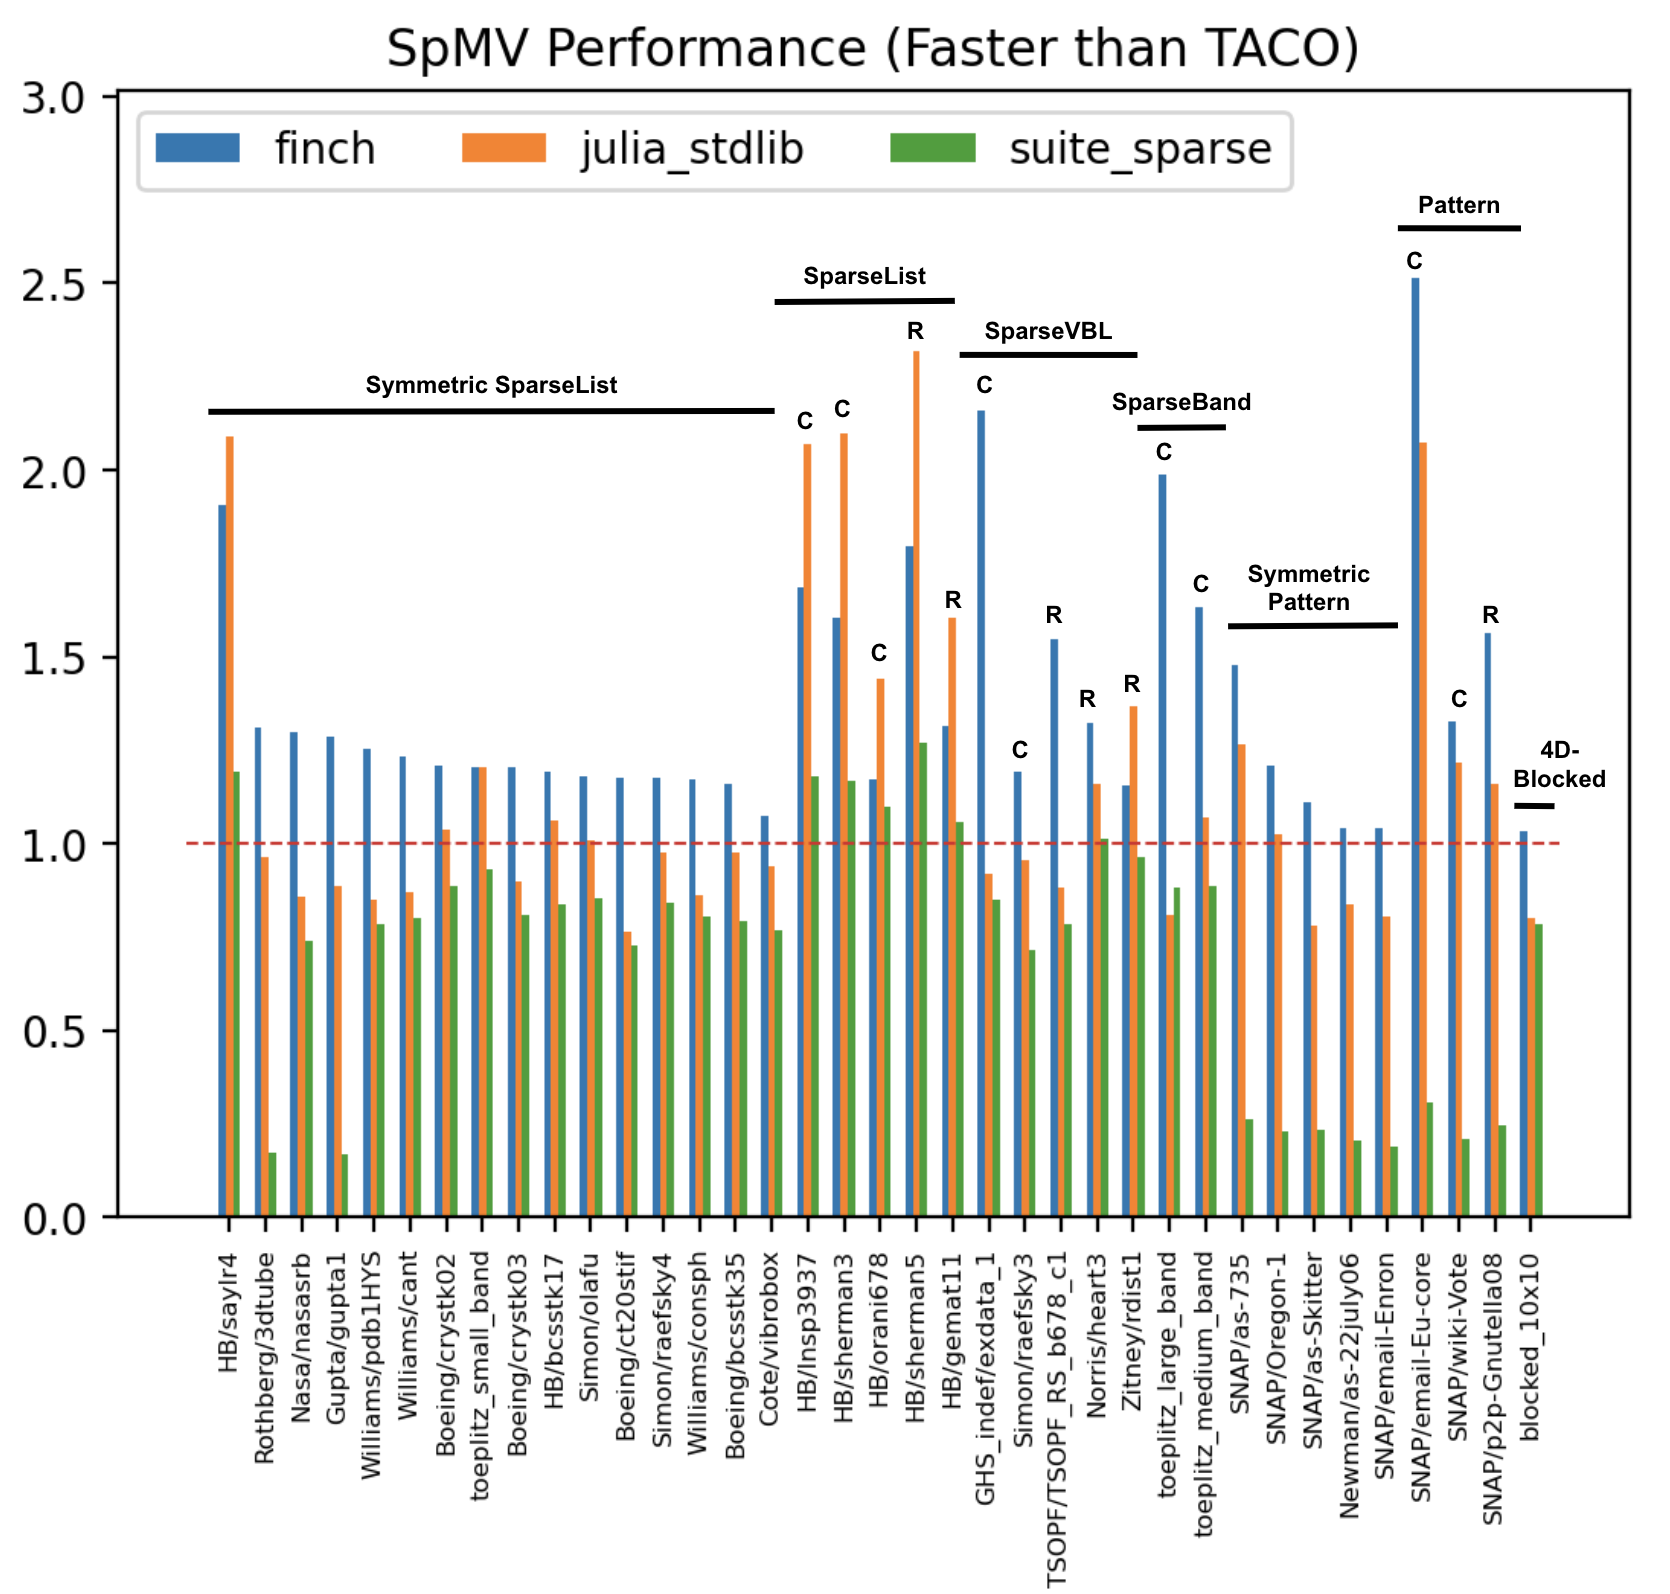
\includegraphics[width=\linewidth]{spmv_performance_grouped.png}
    \caption{Performance of SpMV by Finch format.}
\end{figure}


\subsection{Programming over flexible data}

\subsubsection{Image Morphology}

\begin{figure}
	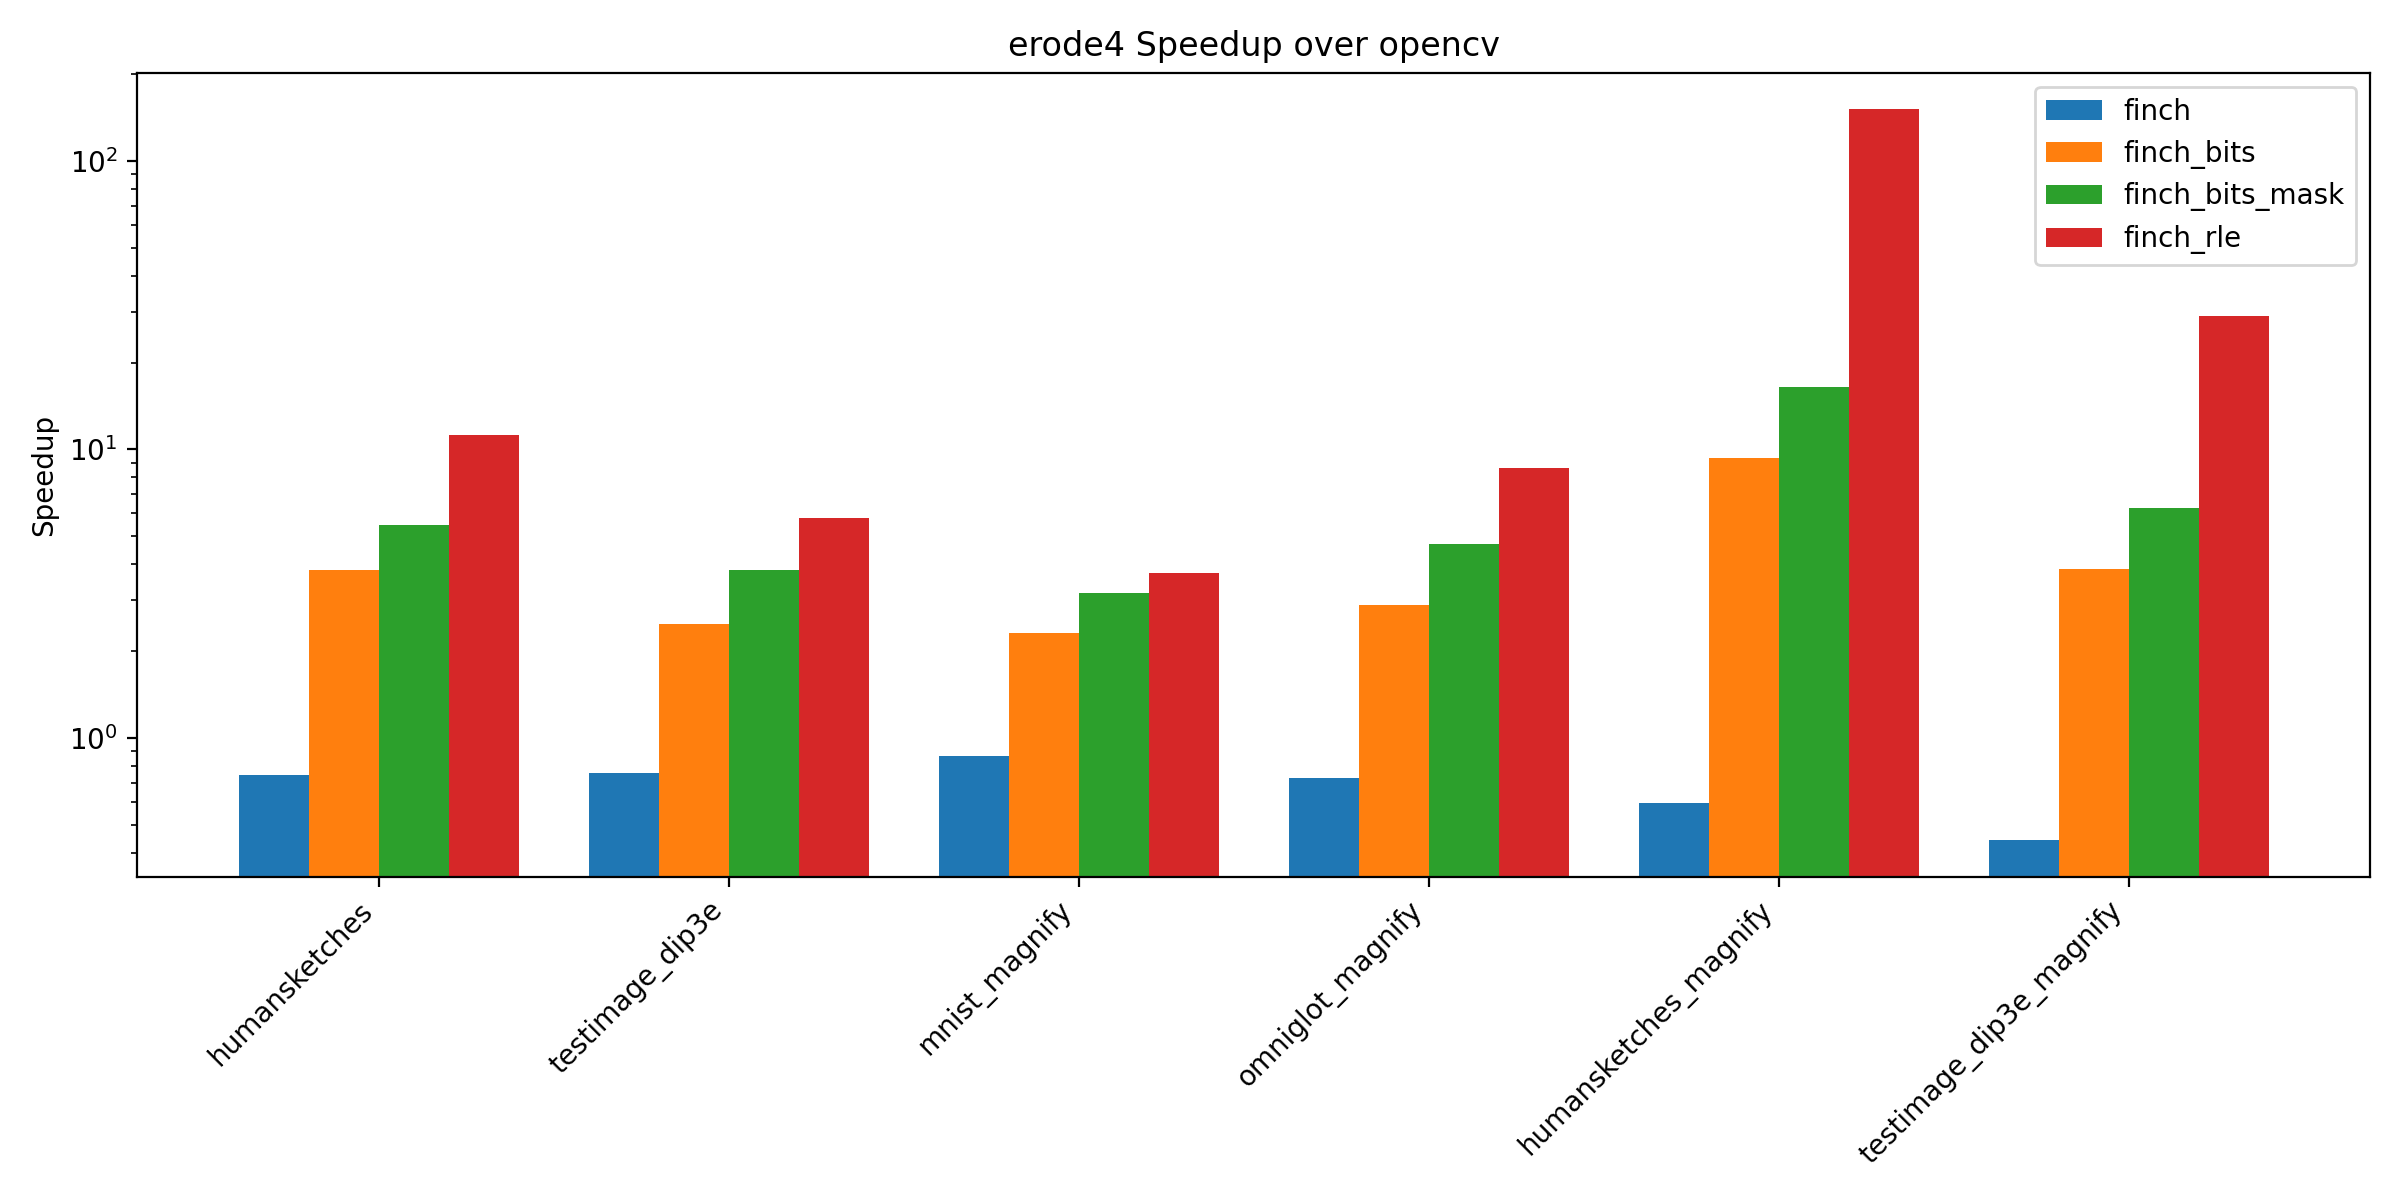
\includegraphics[width=\linewidth]{erode4_speedup_over_opencv.png}
    \caption{Performance of Finch on erosion task (4 iterations).}
\end{figure}

\begin{figure}
	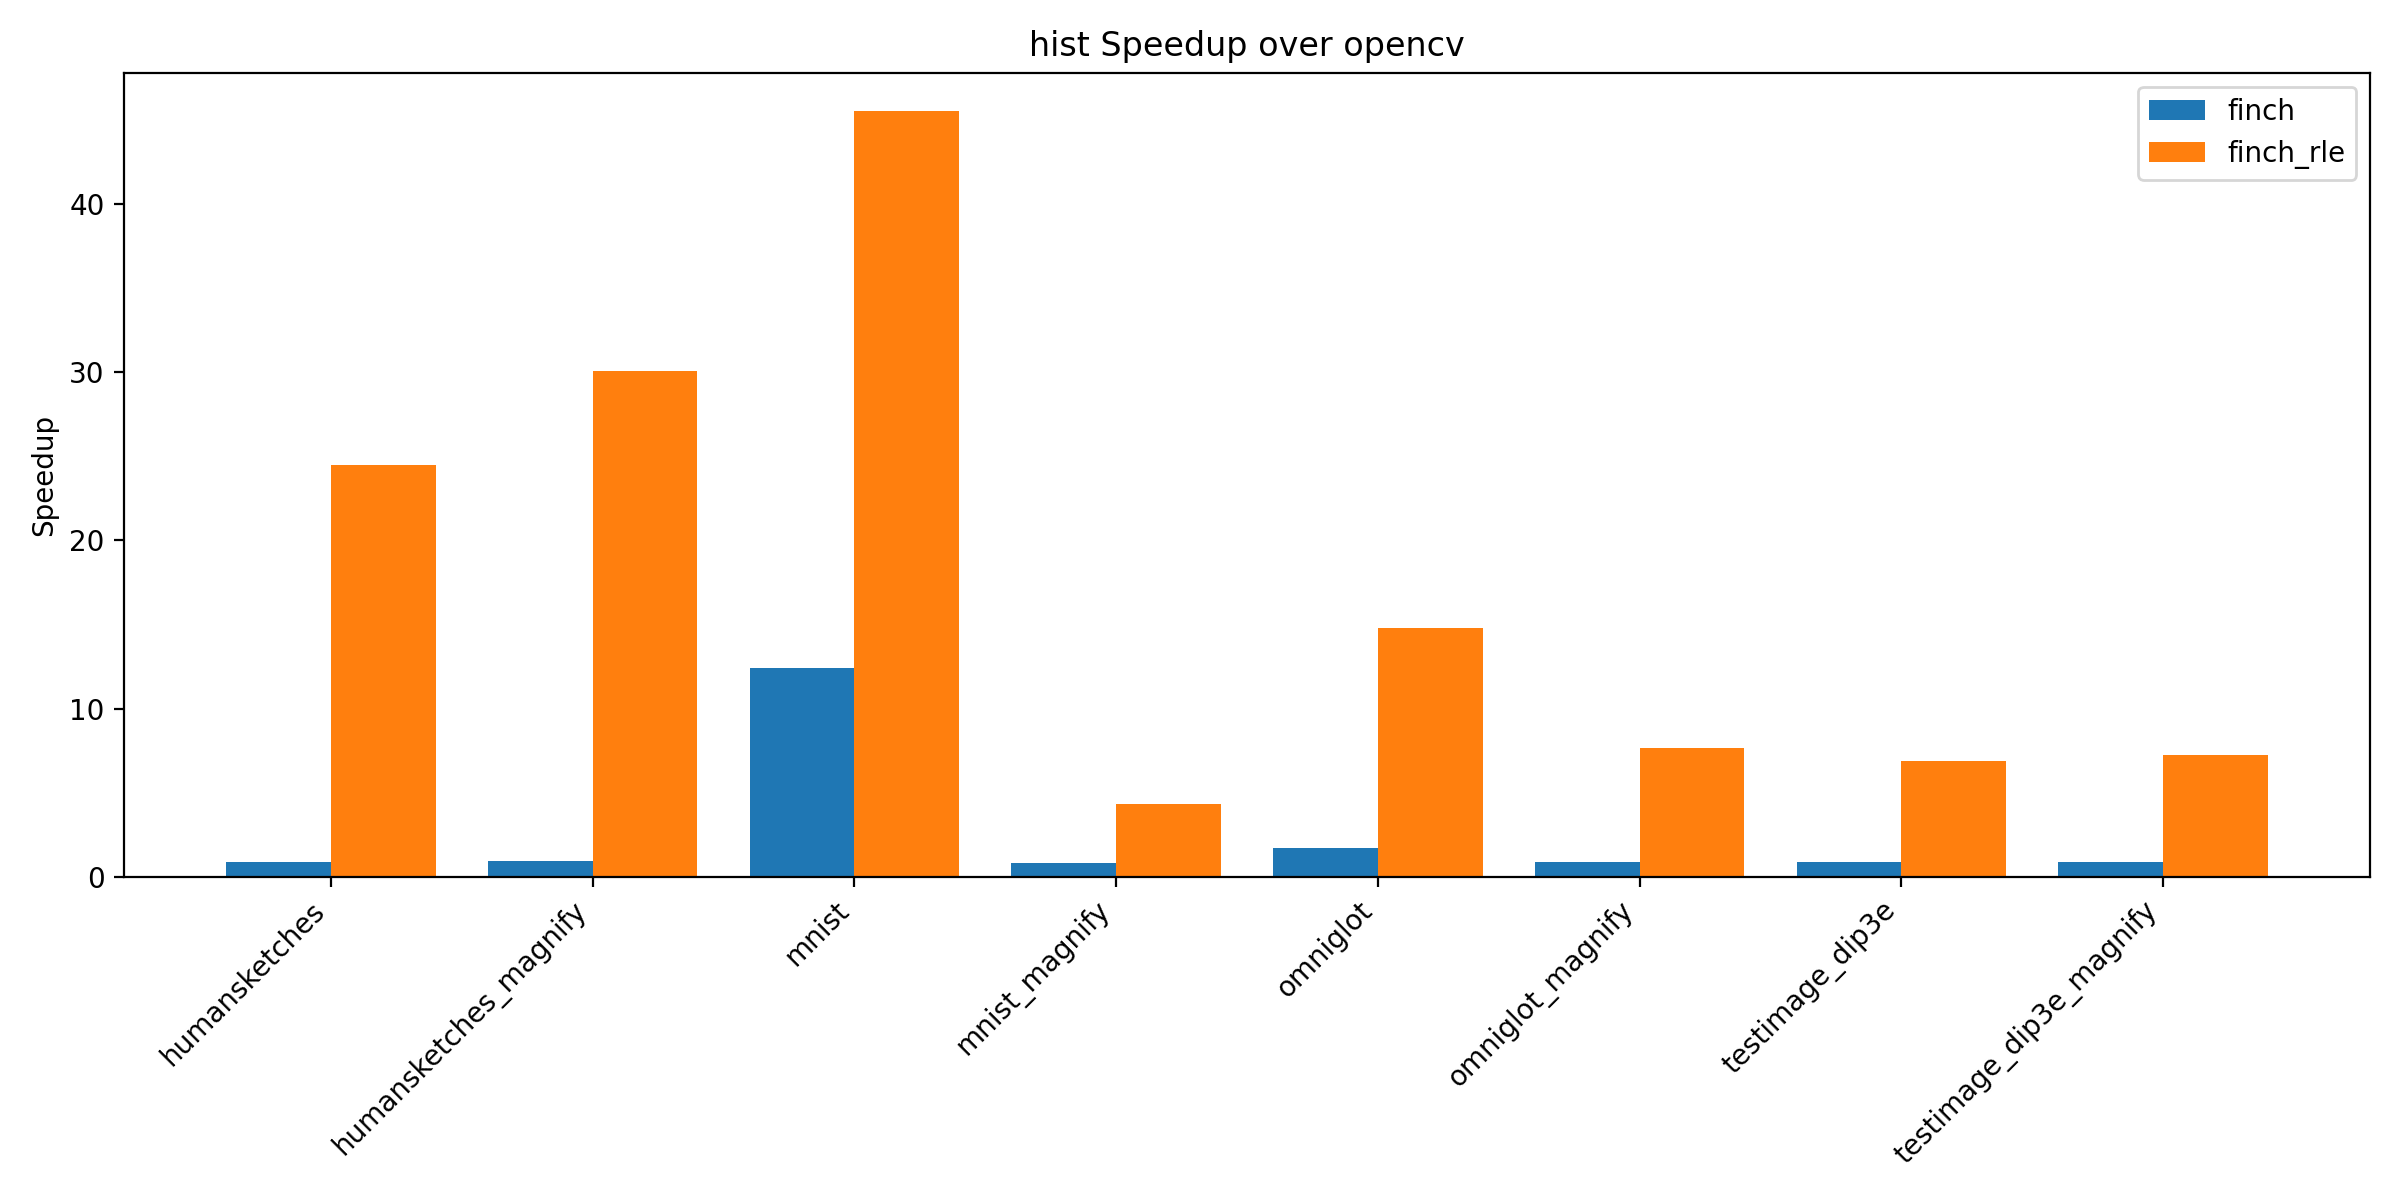
\includegraphics[width=\linewidth]{hist_speedup_over_opencv.png}
    \caption{Performance of Finch on masked histogram task.}
\end{figure}

\begin{figure}
	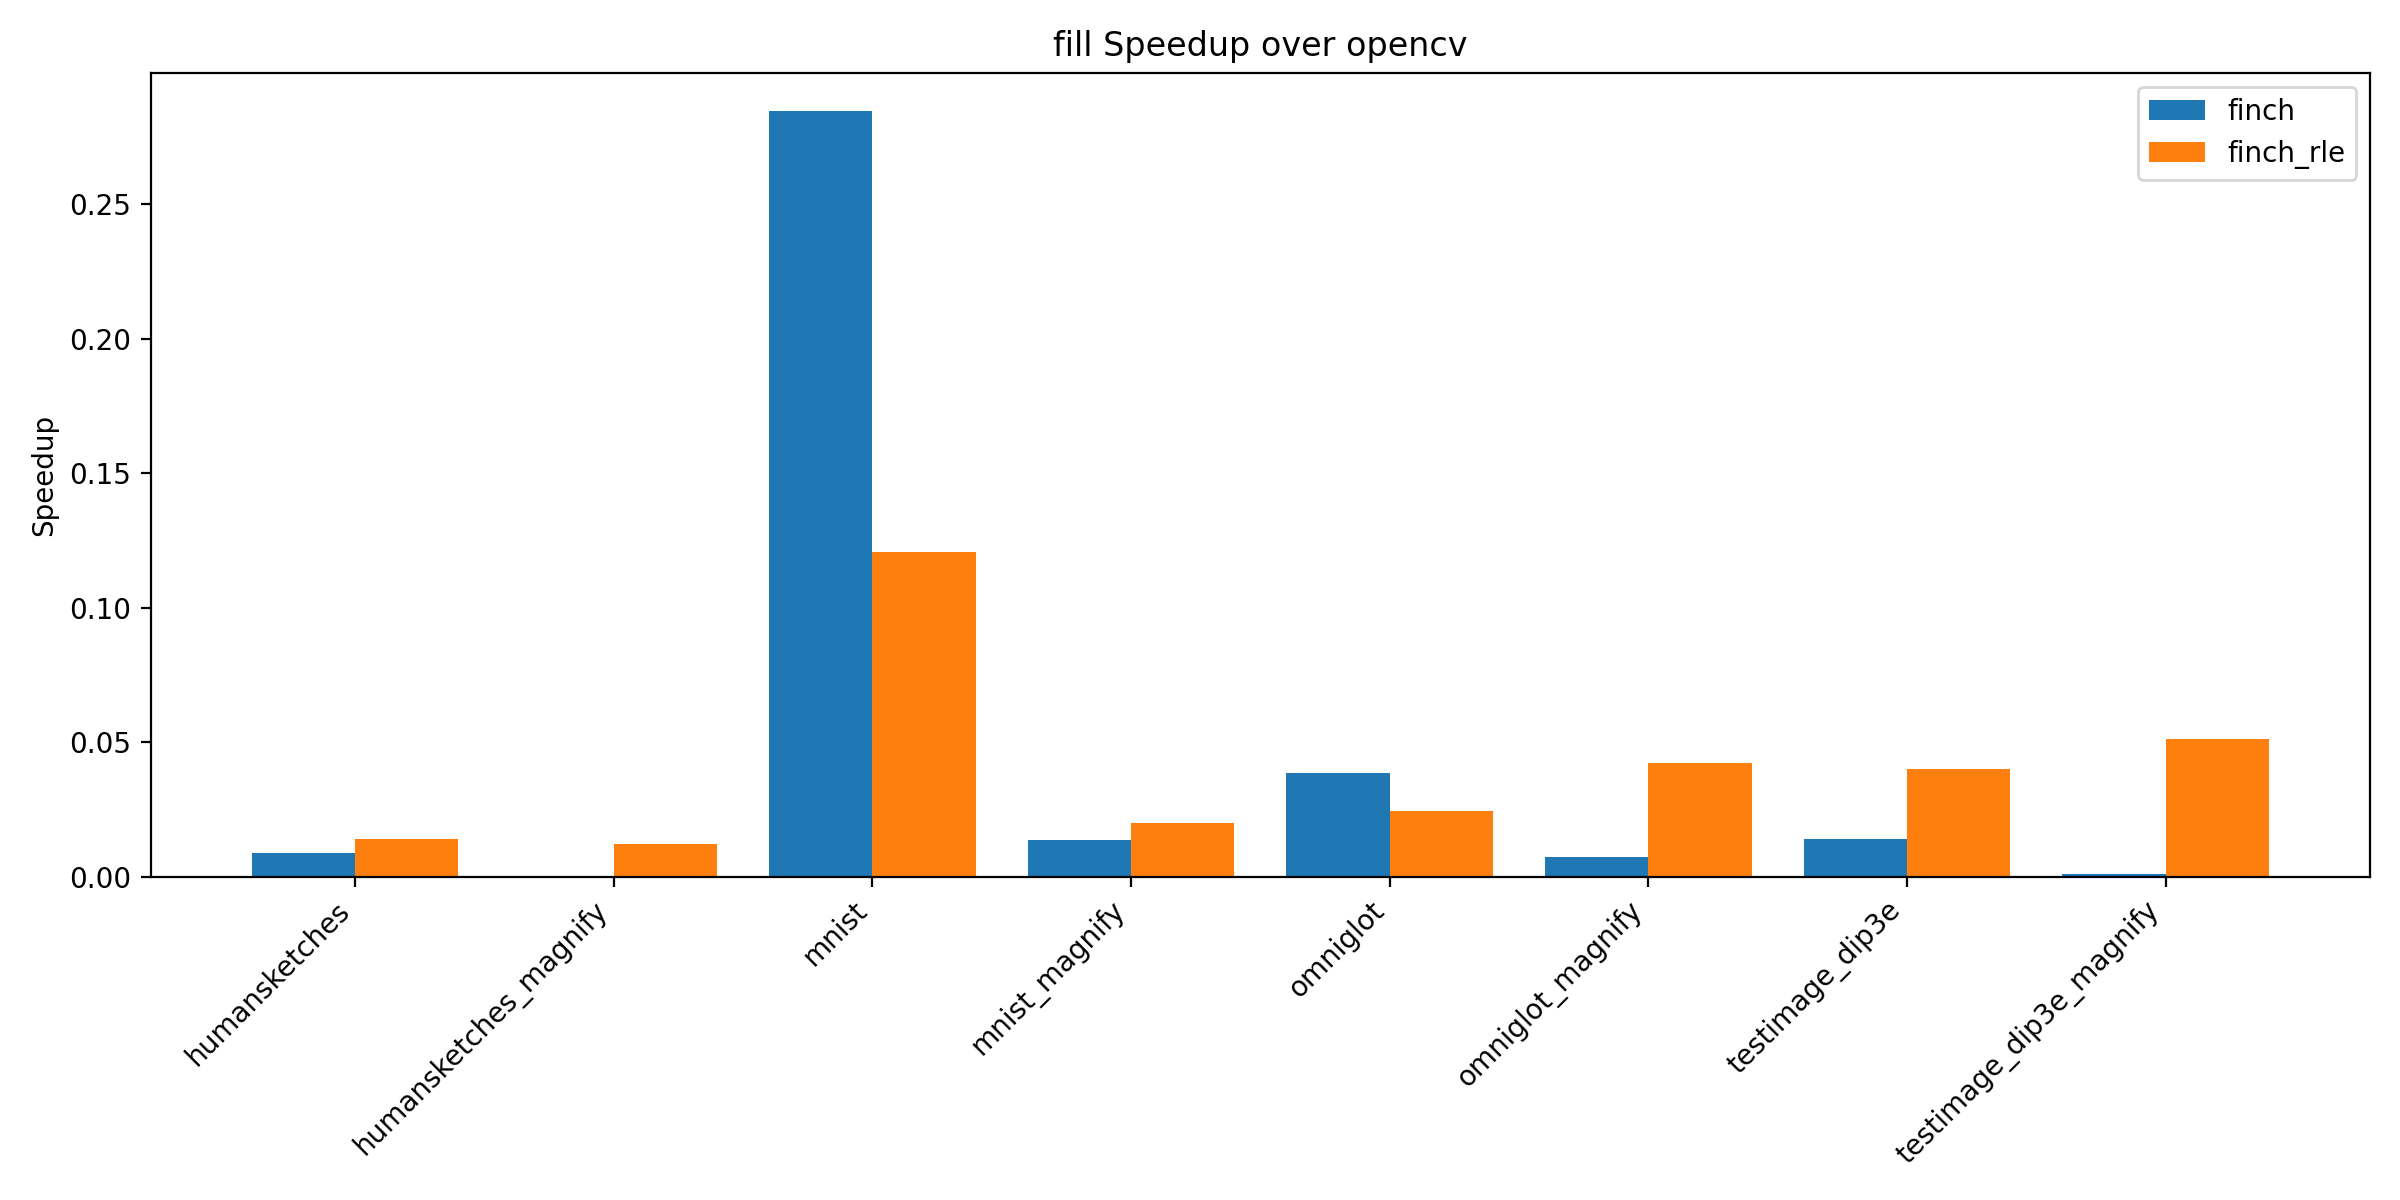
\includegraphics[width=\linewidth]{fill_speedup_over_opencv.png}
    \caption{Performance of Finch on flood fill task.}
\end{figure}

\subsubsection{Graph Analytics}
\begin{figure}
	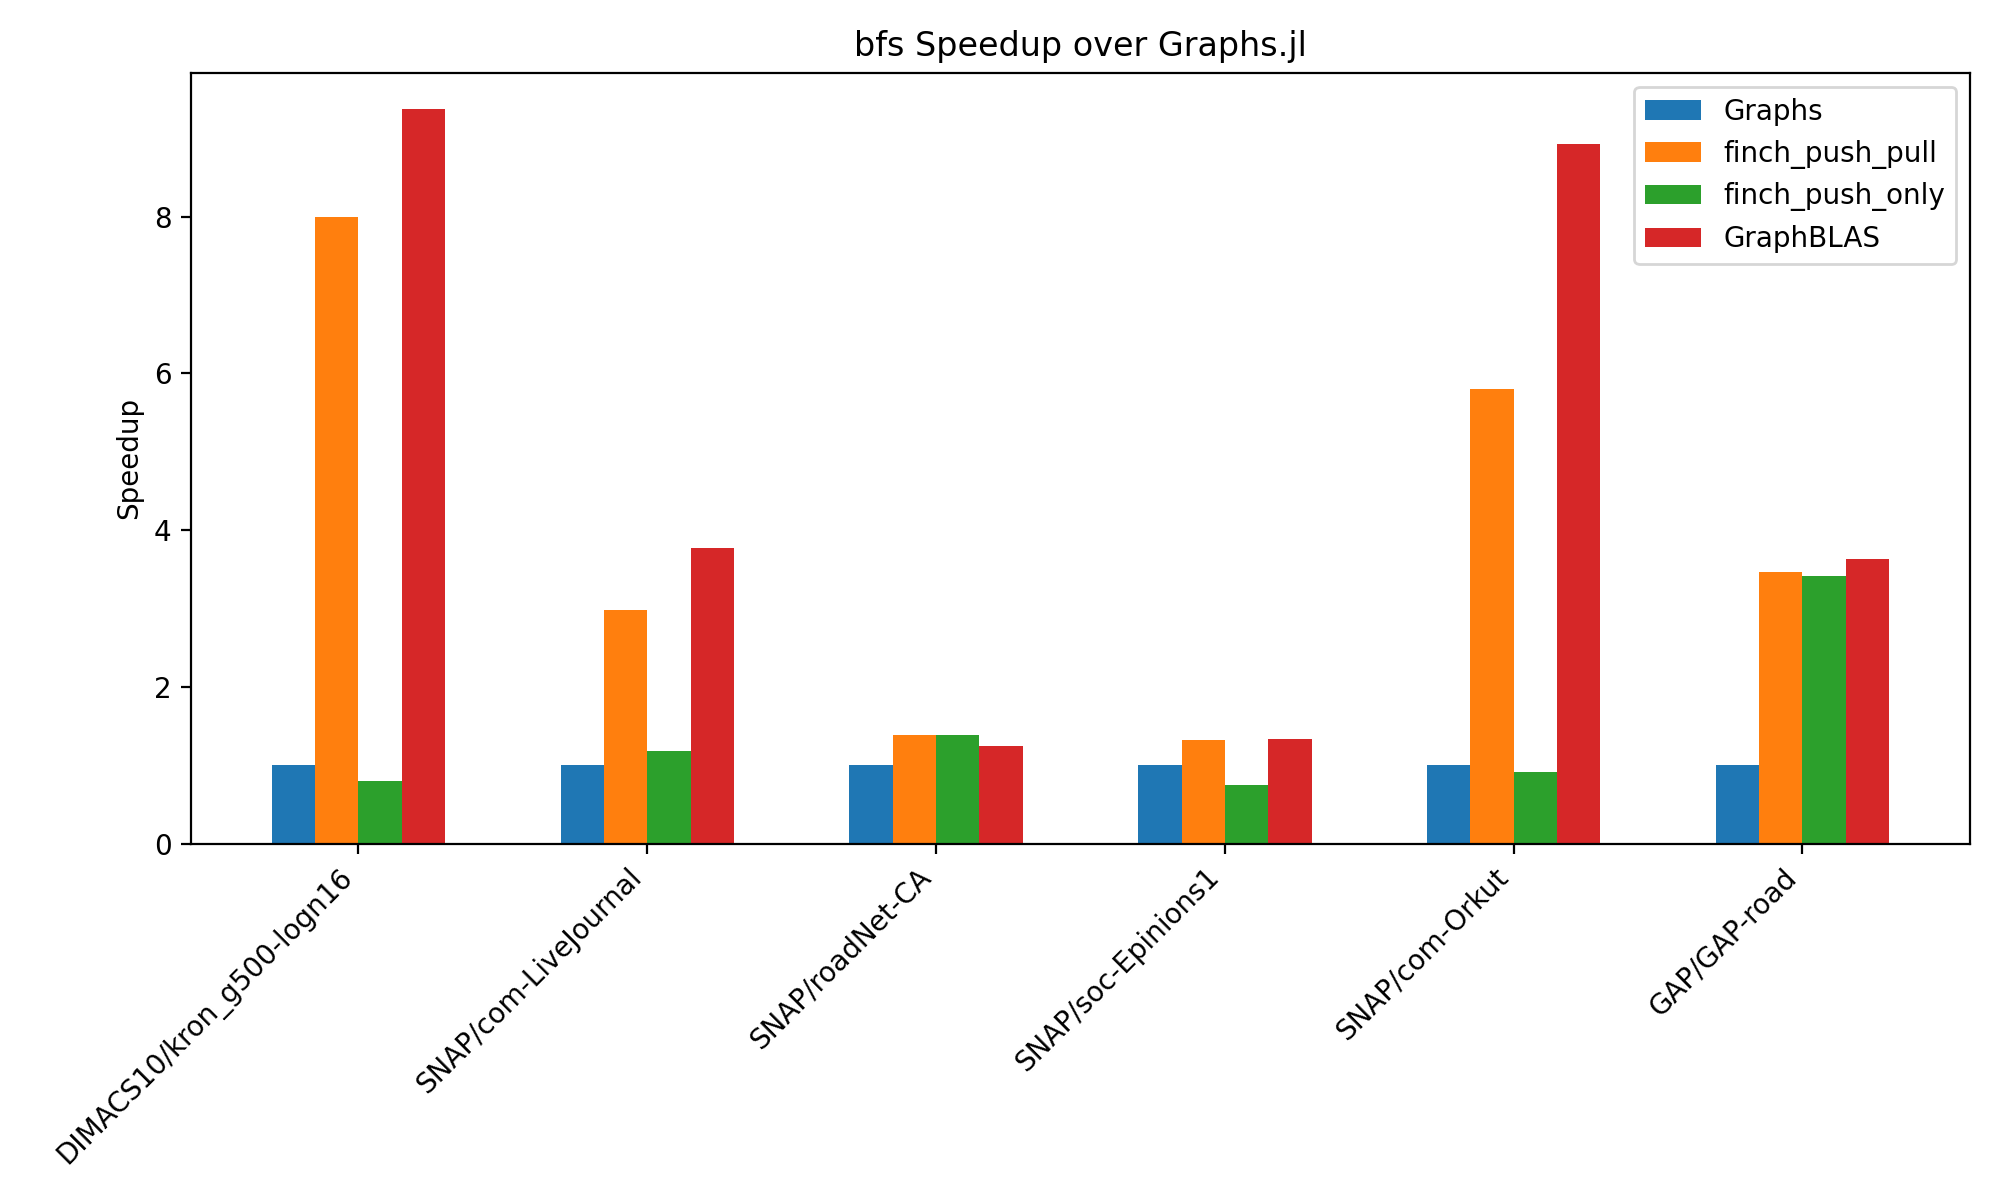
\includegraphics[width=\linewidth]{bfs_speedup_over_graphs.jl.png}
	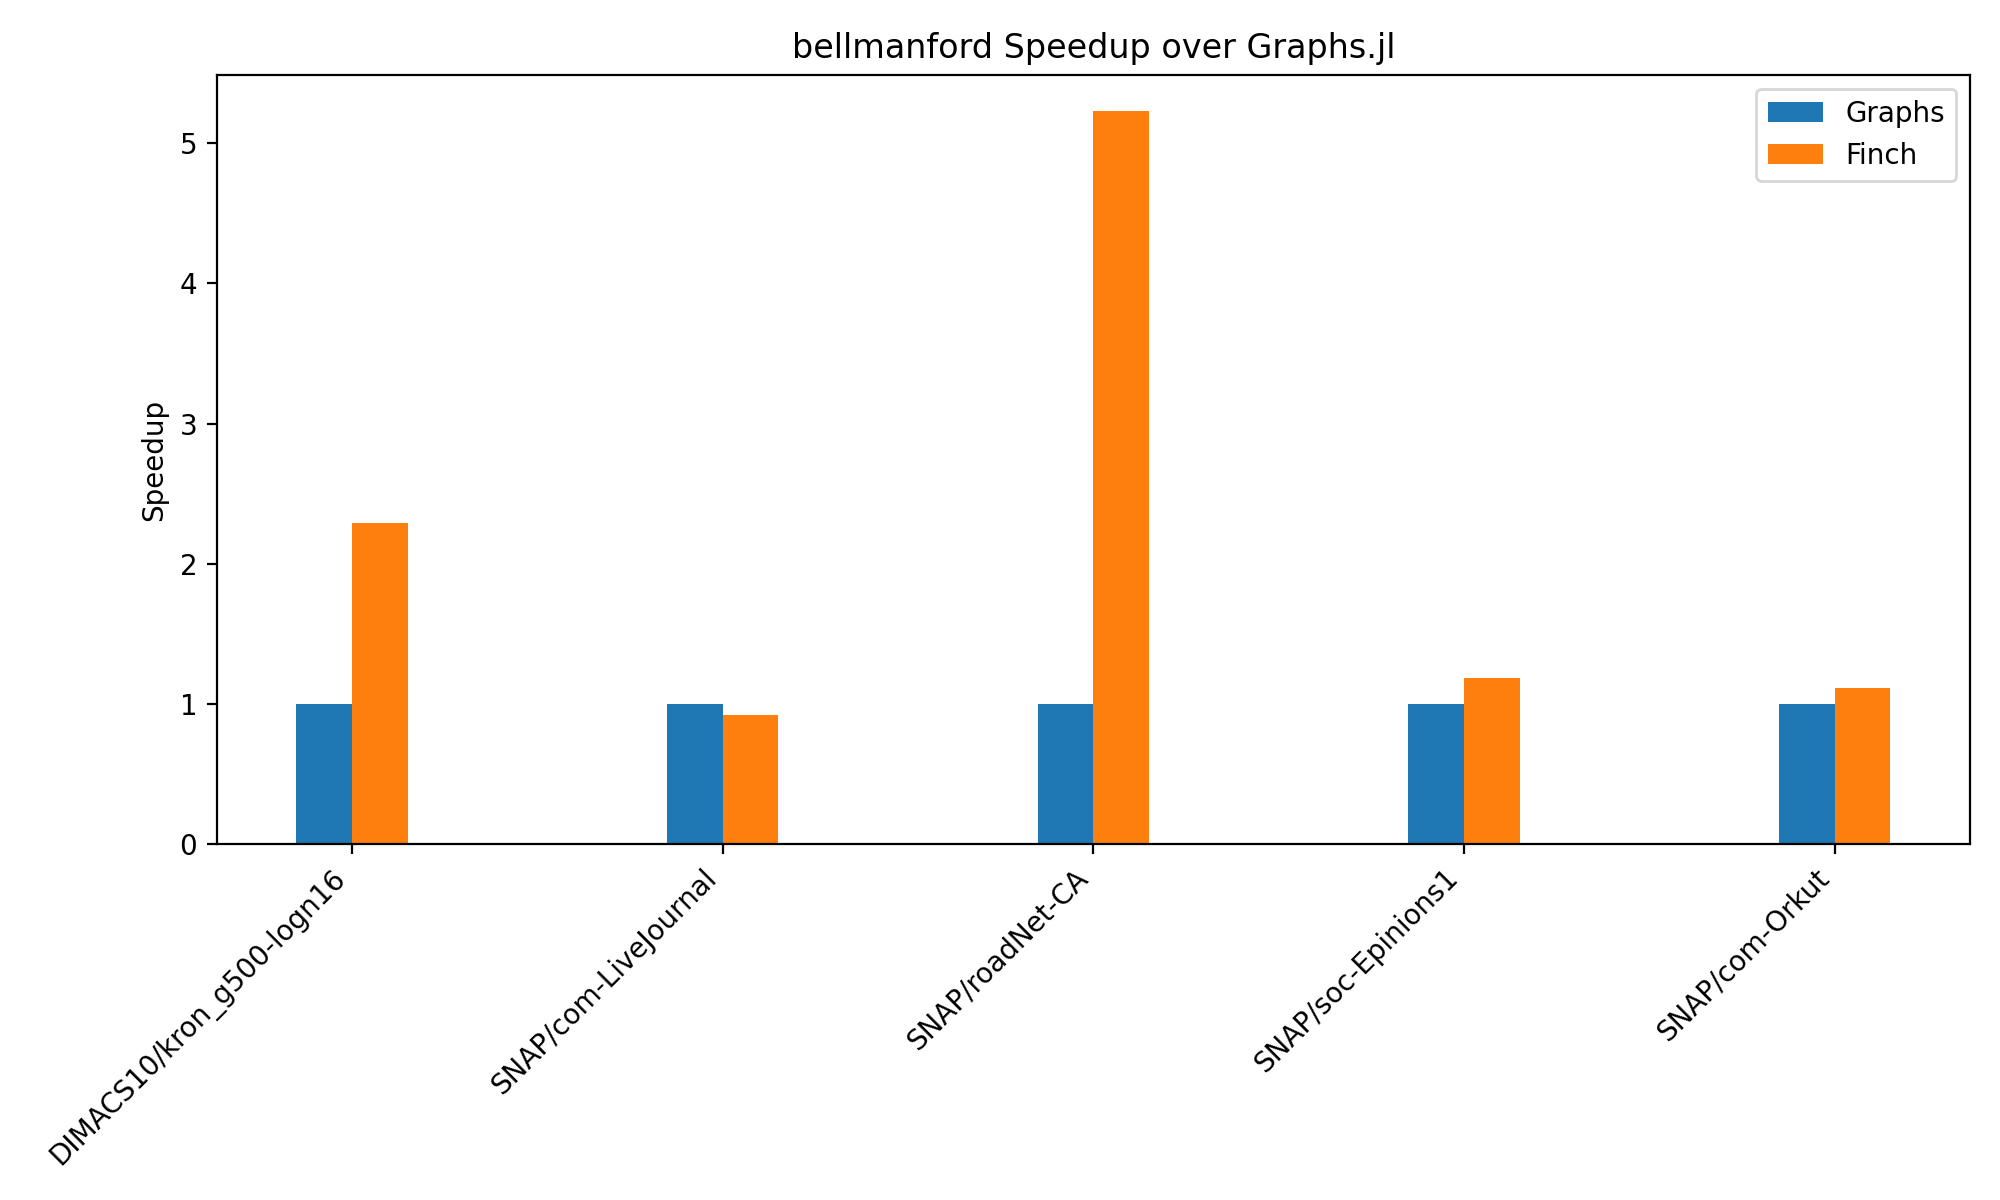
\includegraphics[width=\linewidth]{bellmanford_speedup_over_graphs.jl.png}
    \caption{Performance of graph apps across various tools.}
\end{figure}

\subsubsection{High-level kernel fusion}
Find an example where fusing the python interface gives a big speedup over non-fused kernels.

%%
%% The acknowledgments section is defined using the "acks" environment
%% (and NOT an unnumbered section). This ensures the proper
%% identification of the section in the article metadata, and the
%% consistent spelling of the heading.
\begin{acks}
    To Mateusz, Hameer, and Jaeyeon for their excellent programming contributions to the Finch codebase.
\end{acks}

%%
%% The next two lines define the bibliography style to be used, and
%% the bibliography file.
\bibliographystyle{ACM-Reference-Format}
\bibliography{bibliography.bib}


%%
%% If your work has an appendix, this is the place to put it.
\appendix

\end{document}
\endinput